\documentclass{article}

\PassOptionsToPackage{numbers,sort&compress}{natbib}

% Submission mode: omit final and preprint for anonymized review.
\usepackage{neurips_2026}

\usepackage[utf8]{inputenc}
\usepackage[T1]{fontenc}
\usepackage{hyperref}
\usepackage{url}
\usepackage{booktabs}
\usepackage{amsfonts}
\usepackage{amsmath}
\usepackage{nicefrac}
\usepackage{microtype}
\usepackage{xcolor}
\usepackage{graphicx}
\usepackage{float}
\usepackage{placeins}
\usepackage{array}
\hypersetup{hidelinks}

\title{AtomWorld-Mirror: Macro-Step World Modeling of Critical Evolution Backbones for Materials Dynamics}

\author{%
  \normalfont
  \textbf{Ziming Pan}$^{1,2,*}$ \quad
  \textbf{Ruge Zhang}$^{1,4,5,*}$ \quad
  \textbf{Haozhi Han}$^{1,3}$ \\
  \textbf{Yifeng Chen}$^{3}$ \quad
  \textbf{Yunquan Zhang}$^{4}$ \quad
  \textbf{Ting Cao}$^{1}$ \quad
  \textbf{Yunxin Liu}$^{1}$ \quad
  \textbf{Kun Li}$^{1,\dagger}$ \\
  {\small $^1$Institute for AI Industry Research (AIR), Tsinghua University, Beijing, China}\\
  {\small $^2$Yonsei University, Seoul, Republic of Korea}\\
  {\small $^3$School of Computer Science, Peking University, Beijing, China}\\
  {\small $^4$Institute of Computing Technology, Chinese Academy of Sciences, Beijing, China}\\
  {\small $^5$School of Computer Science and Technology, University of Chinese Academy of Sciences, Beijing, China}\\
  {\small $^*$Equal contribution. \quad $^\dagger$Corresponding author.}\\
  {\small \texttt{likun@air.tsinghua.edu.cn}}
}

\begin{document}

\maketitle

\begin{abstract}
  Atomistic materials simulation is an important computational tool for understanding long-term materials behavior, including diffusion, defect evolution, interfacial reactions, and crack propagation. Many traditional simulators are constrained to advance at microscopic evolutionary resolution: before reaching structurally decisive states, much of the budget is consumed by low-impact local updates. We characterize this as an evolutionary-resolution bottleneck and propose AtomWorld-Mirror, a time-aware macro-step world modeling approach for the critical evolution backbone of atomic systems. AtomWorld-Mirror does not reproduce every microscopic event. Instead, it learns physically reachable macro-step transitions between key states while jointly predicting sparse structural edits and accumulated physical time. We instantiate this modeling approach for event-driven atomistic simulation and use a world model to learn latent macro-step dynamics from short micro-event segments. The model is constrained by local reachability, inventory conservation, and continuous-time consistency. By amortizing local atomic physics into a reusable latent macro model and replacing explicit micro-event replay with macro-step inference, this formulation provides a path toward substantially faster prediction of long-term materials evolution while preserving structural validity and time semantics.
\end{abstract}

\section{Introduction}

Conventional atomistic simulation methods usually describe materials evolution through explicit time stepping or micro-event updates~\cite{alder1959md,verlet1967fluids,bortz1975nfold,gillespie1976general,fichthorn1991dmc}. This stepwise formulation treats different state changes uniformly, even though they play different roles in long-horizon evolution. Some changes are only transient fluctuations, while others accumulate into persistent structural progress. Figure~\ref{fig:key-evolution-budget} illustrates this mismatch in teacher Cu--Fe aging trajectories: Cu-vacancy exchange events that mark key structural evolution appear sparsely and at seed-dependent times within the same fixed replay budget. As a result, standard simulators may spend substantial budget on low-impact intermediate states before reaching structurally consequential configurations in long-horizon evolution~\cite{voter2002timescale,henkelman2000neb,laio2002metadynamics,bolhuis2002tps,soisson1996cufe,soisson2007cufe}. Thus, long-horizon modeling should compress low-impact intermediate states and retain the sparse transitions that carry persistent structural progress; we call this sequence the critical evolution backbone.

Yet, identifying the critical evolution backbone requires looking beyond the current microscopic update. Local simulation can resolve which events are physically valid and how much time they consume, but it does not tell us where a long-horizon rollout should jump: the next retained state must be one that constrains subsequent structural evolution, not merely the next configuration a valid trajectory happens to visit. The model must therefore look ahead from the current configuration, select the next physically reachable waypoint on the backbone, and estimate the physical time accumulated along that transition.

To endow atomistic rollout with this look-ahead ability, we propose AtomWorld-Mirror, an atomistic world model that mirrors atomic evolution in a backbone-imagining latent representation, where rollouts use the inferred backbone to advance rapidly toward long-horizon states rather than replaying every microscopic event~\cite{kingma2014vae,hafner2019planet,hafner2020dreamer,hafner2025dreamer4}. Here, Mirror means that the model does not copy the microscopic trajectory itself, but learns a latent counterpart of atomic evolution that preserves the future-relevant backbone and its physical constraints. Operationally, each rollout step infers the next backbone transition from the current configuration, decodes it into a reachable sparse edit, and predicts the physical time accumulated along that transition~\cite{fichthorn1991dmc,chatterjee2007kmc}. This yields a compressed but physically constrained state-time rollout for long-horizon structural prediction.

In short, the compressed rollout preserves reachability, inventory, and time through three mechanisms: (i) \emph{Local Reachability}. A macro-step prediction cannot be an unconstrained dense reconstruction, because only atomic sites touched by locally reachable microscopic moves can change under the AtomWorld dynamics. Therefore, AtomWorld-Mirror restricts structural prediction to candidate supports derived from the AtomWorld teacher and applies a projected forward path during training and rollout. (ii) \emph{Inventory Conservation}. Although local reachability limits where edits may occur, a macro edit can still violate material validity if it changes the inventory of atoms and vacancies. Our projection-closed sparse-edit formulation therefore preserves material inventory while converting latent macro predictions into lattice edits. (iii) \emph{Continuous-Time Consistency}. Physical duration is therefore predicted as a path-conditioned quantity, using AtomWorld path summaries during training and prior path latents during rollout, because related macro endpoints can accumulate different waiting-time scales along different microscopic paths~\cite{gillespie1976general,gillespie1977exact,fichthorn1991dmc}. Empirically, across controlled long-horizon materials-simulation diagnostics, AtomWorld-Mirror captures backbone-level sparse state changes through physically valid edits, aligns path-conditioned time and energy/reward predictions along teacher trajectories, and yields tens-to-hundreds-fold speedups in a timed end-to-end diagnostic against event-by-event simulation. Thus, the reported gain is not only faster rollout; it reflects a macro world model that preserves the state, energy, and time semantics needed for long-horizon materials evolution.

\begin{figure}[H]
  \centering
  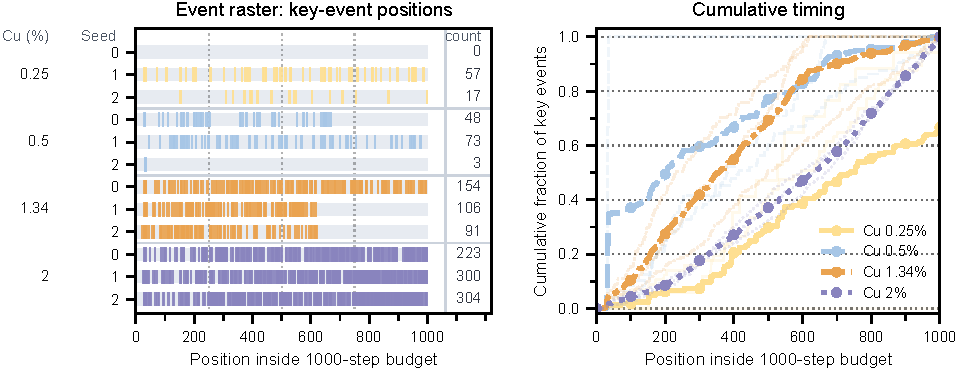
\includegraphics[width=0.92\linewidth]{fig/fig1_key_evolution_budget_randomness.pdf}
  \caption{Random timing of key structural evolution within a fixed kinetic simulator replay budget. Each row is one kinetic simulator trajectory at a specified Cu density and random seed; ticks mark Cu-vacancy exchange events within a $1000$-micro-event budget, and the cumulative curves show how these events accumulate across the budget.}
  \label{fig:key-evolution-budget}
\end{figure}

\section{Problem formulation}

\subsection{Micro-event resolution and key-state evolution}

% Let $X_t$ denote the atomic configuration after the $t$-th microscopic update, with an associated physical clock $T_t$. A traditional simulator resolves a fine-grained trajectory~\cite{verlet1967fluids,plimpton1995fast,thompson2022lammps,bortz1975nfold,gillespie1977exact}
% \begin{equation}
% X_0 \rightarrow X_1 \rightarrow X_2 \rightarrow \cdots \rightarrow X_N,
% \end{equation}
% where each transition is a local update, integration step, or atom-vacancy event. These updates are physically meaningful, but long-term material behavior is often governed by a much smaller set of structurally decisive states~\cite{voter2002timescale,henkelman2000neb,laio2002metadynamics,bolhuis2002tps,soisson1996cufe,soisson2007cufe}. The simulator can check local validity, but validity alone does not decide whether a state should be retained for long-horizon prediction.


Let \(X_t\) denote the atomic configuration after the \(t\)-th microscopic
update, with associated physical clock \(T_t\). A traditional simulator resolves
a fine-grained trajectory \(\{X_t\}_{t=0}^{N}\), where each transition
\(X_t\to X_{t+1}\) is a local update, integration step, or atom-vacancy event
~\cite{verlet1967fluids,plimpton1995fast,thompson2022lammps,bortz1975nfold,gillespie1977exact}.
These updates are physically meaningful, but long-term material behavior is
often governed by a much smaller set of structurally decisive states
~\cite{voter2002timescale,henkelman2000neb,laio2002metadynamics,bolhuis2002tps,soisson1996cufe,soisson2007cufe}.
The simulator can check local validity, but validity alone does not decide
whether a state should be retained for long-horizon prediction.

We denote a sparse key-state subsequence by
\begin{equation}
\mathcal{B}=(X_{n_0},X_{n_1},\ldots,X_{n_M}), \quad 0=n_0<n_1<\cdots<n_M\leq N,
\end{equation}
with $M\ll N$, and call it the critical evolution backbone. A transition $X_{n_m}\rightarrow X_{n_{m+1}}$ may subsume many microscopic updates while representing one structurally meaningful macro advance, a view related to Semi-Markov temporal abstraction and model-based temporal prediction~\cite{sutton1988td,sutton1990dyna,sutton1999options}. The challenge is predictive selection: learn a macro representation that chooses the next backbone state useful for future structural evolution and estimates its physical duration without replaying every intermediate event.

\subsection{Time-aware macro-step objective}

To make predictive selection trainable, choose a macro horizon $k\in\mathcal{K}$ that counts teacher micro events rather than physical time. A direct full-state objective is
\begin{equation}
p_\theta(X_{t+k},\tau_{t:t+k}\mid X_t,k),
\end{equation}
where $\tau_{t:t+k}$ is the macro duration, e.g., $T_{t+k}-T_t$ for a realized path. This target contains the required state and time objects but is inefficient for lattices because most sites remain unchanged, so we use candidate-restricted edit labels over a physically motivated reachable set $\mathcal{C}_k(X_t)$:
\begin{equation}
\Delta X_{t:t+k}=\{(i,a_i)\}_{i\in\mathcal{C}_k(X_t)},
\end{equation}
where $a_i$ is the final local edit label or occupancy state at candidate site $i$; unchanged candidates copy the current state, so the effective edit remains sparse. Because changing $k$ changes the region teacher dynamics can affect, the modeling objective becomes
\begin{equation}
p_\theta(\Delta X_{t:t+k},\tau_{t:t+k}\mid X_t,\mathcal{C}_k(X_t),k).
\end{equation}
This objective differs from endpoint-only regression in two ways. First, the candidate support is part of the prediction problem: if a site is not reachable under the teacher dynamics at the chosen horizon, changing it would create a plausible-looking but physically unsupported macro state. Second, the duration is coupled to the microscopic path used to reach the endpoint, not only to the endpoint itself. The model must therefore learn a state-time transition whose structural support, endpoint edit, and elapsed physical time are jointly valid.

\subsection{KMC-provided AtomWorld as a continuous-time teacher}

In KMC, the current state $X_t$ has possible events $\mathcal{E}(X_t)=\{e_1,\ldots,e_n\}$ with rates $r_i(X_t)$~\cite{bortz1975nfold,gillespie1976general,fichthorn1991dmc}. The total escape rate is
\begin{equation}
R(X_t)=\sum_i r_i(X_t),
\end{equation}
and event selection and waiting time are
\begin{equation}
p(e_i\mid X_t)=\frac{r_i(X_t)}{R(X_t)}, \qquad \Delta t\sim \mathrm{Exp}(R(X_t)).
\end{equation}
A KMC micro event therefore couples structural change with clock advance, with expected waiting time $1/R(X_t)$ and update $T_{t+1}=T_t+\Delta t_t$. For a teacher segment of $k$ events, define
\begin{equation}
\tau_{\mathrm{exp}}(t,k)=\sum_{j=0}^{k-1}\frac{1}{R(X_{t+j})}, \qquad
\tau_{\mathrm{real}}(t,k)=T_{t+k}-T_t=\sum_{j=0}^{k-1}\Delta t_{t+j}.
\end{equation}
AtomWorld-Mirror uses $\tau_{\mathrm{exp}}$ as the primary macro-time target because it preserves the expected CTMC clock along the teacher path; $\tau_{\mathrm{real}}$ is retained for stochastic-time diagnostics. Thus macro time is a path-conditioned aggregate over encountered rates, not a pure endpoint attribute. KMC is a useful teacher because it provides exact local event semantics, locally valid trajectories, and explicit continuous-time labels~\cite{chatterjee2007kmc}; the same formulation can apply to other event-driven atomistic simulators with sparse structurally important states.

\section{AtomWorld-Mirror}

AtomWorld-Mirror implements the macro transition objective as a teacher-student world model that mirrors atomistic evolution in a backbone-aware latent space rather than replaying every micro event. AtomWorld denotes the teacher-exposed atomic evolution world: configurations, local event support, transition rules, and physical clock. Mirror denotes the student-side macro evolution model over backbone state-time transitions. The teacher supplies short, locally valid state-time segments; the student predicts reachable sparse edits, accumulated duration, and the next macro latent state for selected horizons. Here the teacher is atomistic KMC and the student is a DreamerV4-style latent world model, but any event-driven atomistic teacher and latent world model with sparse structural states and physical-time supervision could instantiate the same split.

\subsection{Teacher supervision}

Given an initial configuration \(X_t\), the teacher advances the underlying
microscopic dynamics over a short segment of horizon \(k\in\mathcal{K}\),
producing the local trajectory \(\{X_{t+i}\}_{i=0}^{k}\)
~\cite{fichthorn1991dmc,chatterjee2007kmc}.
Each supervised macro sample contains
\begin{equation}
(X_t,k,X_{t+k}, \Delta X_{t:t+k}, \tau_{\mathrm{exp}}, \tau_{\mathrm{real}}, s_{\mathrm{path}}, \mathcal{C}_k).
\end{equation}
Here $\mathcal{K}$ is the controlled Multi-K horizon set, $\Delta X_{t:t+k}$ is the start-to-end sparse edit, $s_{\mathrm{path}}$ summarizes the microscopic path, and $\mathcal{C}_k$ is the reachable candidate set. The teacher supervises a state-time macro transition rather than a single next-state label: endpoint for what changed, path summary for how it was reached, and duration targets separating expected CTMC time from sampled waiting-time noise. Such path-derived supervision follows the atomistic KMC view used in vacancy-mediated alloy studies~\cite{soisson1996cufe,soisson2007cufe}. The realized duration is
\begin{equation}
\tau_{\mathrm{real}}=\sum_{j=0}^{k-1}\Delta t_{t+j},
\end{equation}
while the primary time target is the path-conditioned accumulated expected time
\begin{equation}
\tau_{\mathrm{exp}}=\sum_{j=0}^{k-1}\frac{1}{R(X_{t+j})}.
\end{equation}
We use $\tau_{\mathrm{exp}}$ as main duration supervision because it reflects the expected CTMC clock without exponential waiting-time noise. $\tau_{\mathrm{real}}$ remains an auxiliary stochastic target and time-uncertainty diagnostic. During data construction, unchanged start--end segments are skipped because they confound sparse-edit learning and macro-duration calibration; remaining samples require an actual reachable structural change.

Supervised segments become student rollouts through three physical commitments. (i) \textbf{Local Reachability}. Macro prediction is not dense reconstruction: only sites touched by locally reachable moves can change, so AtomWorld-Mirror restricts edits to teacher-derived candidate supports and uses a projected forward path during training and rollout. (ii) \textbf{Inventory Conservation}. Reachability limits edit locations, but projection-closed sparse edits must also preserve atom and vacancy inventory while converting latent predictions into lattice edits. (iii) \textbf{Continuous-Time Consistency}. Physical duration is path-conditioned, using AtomWorld path summaries in training and prior path latents in rollout because related endpoints can accumulate different waiting-time scales~\cite{gillespie1976general,gillespie1977exact,fichthorn1991dmc}. The following subsections implement these commitments through latent dynamics, sparse-edit projection, and duration losses.

\subsection{Student latent world model}

The student builds on Dreamer-style latent world modeling, with DreamerV4 as the implementation line for scalable latent rollout~\cite{hafner2019planet,hafner2020dreamer,hafner2021dreamerv2,hafner2025dreamer4}, and on related model-based RL ideas~\cite{deisenroth2011pilco,nagabandi2018neuralmb,chua2018pets,janner2019mbpo,kaiser2020atari}, adapted from action-conditioned control to teacher-supervised atomistic macro transitions. It encodes the current configuration and context using latent-variable, graph-simulator, and molecular message-passing ideas~\cite{kingma2014vae,battaglia2016interaction,sanchez2018physics,kipf2018nri,sanchez2020learning,pfaff2021meshgraphnets,gilmer2017mpnn,kipf2017gcn,velickovic2018gat,xu2019gin,gasteiger2020dimenet,satorras2021egnn,fuchs2020se3},
\begin{equation}
z_t=\mathrm{Enc}_\theta(X_t,g_t),
\end{equation}
where $g_t$ may contain local composition, defect statistics, rate summaries, vacancy information, or other global context. The active-patch encoder also produces site embeddings for $\mathcal{C}_k(X_t)$, so global latent dynamics and local edit space are learned jointly. Because the same $X_t$ can lead to different reachable endpoints and $k$ changes the admissible path family, AtomWorld-Mirror introduces a horizon-conditioned path latent $h_t$.

During training, the posterior path latent can condition on the endpoint and the teacher path summary,
\begin{equation}
q_\phi(h_t\mid z_t,z_{t+k},s_{\mathrm{path}},k),
\end{equation}
which makes the supervised transition identifiable. During inference, endpoint and teacher path are unavailable, so the model samples or selects from a prior
\begin{equation}
p_\theta(h_t\mid z_t,g_t,k).
\end{equation}
The macro dynamics then predicts a horizon-conditioned next latent,
\begin{equation}
\hat{z}_{t+k}=z_t+F_\theta(z_t,h_t,k).
\end{equation}
A KL term aligns prior and posterior, enabling test-time macro rollout from the current state alone: the posterior uses teacher information for identifiable training, while the prior is the rollout-time path representation.
This separation avoids a training--inference mismatch. Endpoint-conditioned supervision alone could make the edit decoder accurate only when teacher paths are visible, while prior-only early training would leave several reachable macro outcomes ambiguous. The posterior/prior pair lets the teacher explain which path was taken during learning while requiring deployed rollout to predict the path latent from the current state and horizon.

\subsection{Reachability-constrained sparse edits}

The edit decoder is defined over $\mathcal{C}_k(X_t)$, not the full lattice. Candidate-restricted event supports are standard in spatial and adaptive KMC~\cite{chatterjee2007kmc,henkelman2001akmc,zamora2016spectad}, with related barrier/path-based rare-event context in NEB and time-reversal path-sampling work~\cite{henkelman2000neb,liu2023trps}. For candidate site $i$, the decoder takes site embedding $u_i$, patch context, predicted macro latent $\hat{z}_{t+k}$, path latent $h_t$, and horizon $k$, and predicts change logit $\ell_i$ and final type distribution $\pi_i$,
\begin{equation}
(\ell_i,\pi_i)=D_\theta(u_i,\hat{z}_{t+k},h_t,k).
\end{equation}
Let $m_i=\mathbf{1}\{x_{t+k,i}\neq x_{t,i}\}$ be the teacher change mask and $a_i$ be the target final type. A compact sparse-edit loss is
\begin{equation}
\mathcal{L}_{\mathrm{edit}}
=
-\sum_{i\in\mathcal{C}_k(X_t)}
\left[
m_i\log\sigma(\ell_i)
+(1-m_i)\log(1-\sigma(\ell_i))
+\beta m_i\log \pi_i(a_i)
\right],
\end{equation}
where the first two terms learn sparse support and the last learns changed-site type. Candidate restriction is part of the output space, not cosmetic post-processing: it removes unchanged regions and prevents arbitrary unreachable edits, which is crucial for vacancy-mediated alloy evolution where hops, composition, and trapping jointly determine feasible changes~\cite{soisson1996cufe,soisson2007cufe}.

Inventory conservation further requires the candidate patch to preserve material counts:
\begin{equation}
\sum_{i\in\mathcal{C}_k(X_t)}\mathbf{1}\{\hat{x}_{t+k,i}=c\}
=
\sum_{i\in\mathcal{C}_k(X_t)}\mathbf{1}\{x_{t,i}=c\},
\qquad c\in\{\mathrm{Fe},\mathrm{Cu},\mathrm{Vac}\},
\end{equation}
Outside the patch, sites are copied from the current configuration. Projection is implemented as paired vacancy--atom transport, selecting vacancy-to-atom and atom-to-vacancy pairs under the budget
\begin{equation}
d_{\mathrm{vac}}\leq k,\qquad d_{\mathrm{Cu}}\leq k,\qquad d_{\mathrm{vac}}+d_{\mathrm{Cu}}\leq 2k,\qquad |\Delta\hat{X}_{t:t+k}|\leq 2k,
\end{equation}
where distances use the periodic BCC hop metric. The same projected forward path is used during training and inference: projected states are re-encoded for latent, reward, and duration losses, so optimization targets the states actually rolled out. Projection is therefore part of the closed loop rather than a late inference-only repair.
This keeps the edit loss and rollout semantics aligned. A raw decoder can rank candidate changes, but the physically executed macro transition is the projected edit after reachability and inventory constraints are applied. Training downstream losses on the projected state forces latent prediction, reward prediction, and duration prediction to see the same state that will be fed into the next macro step.

\subsection{Continuous-time duration modeling and loss}

Duration is a core macro-transition output, not an auxiliary endpoint property, because stochastic simulation uses the same rates for event selection and waiting time~\cite{gillespie1976general,gillespie1977exact,fichthorn1991dmc,lin2019partialscaling}. We separate path-conditioned expected CTMC duration from realized sampled duration: $\tau_{\mathrm{exp}}$ is the main macro-time target, while $\tau_{\mathrm{real}}$ is auxiliary stochastic supervision.

\noindent The duration branch predicts expected macro time in log space,
\begin{equation}
b_k(X_t)=\log k-\log R(X_t), \qquad
\mu_{\mathrm{exp}}=b_k(X_t)+r^\tau_\theta(z_t,\hat{z}_{t+k},h_t,g_t,\rho_t,k),
\end{equation}
where $b_k(X_t)$ is the log start-state CTMC estimate $k/R(X_t)$, $\rho_t$ is edit/projection context, and $r^\tau_\theta$ is a residual. The residual is needed because the true target is $\sum_j 1/R(X_{t+j})$, not $k/R(X_t)$; the baseline anchors scale while the learned branch corrects path-dependent rate changes. The expected-time head also predicts $\log\sigma_{\mathrm{exp}}$, and the main duration loss is the implementation's log-space Gaussian negative log-likelihood:
\begin{equation}
\mathcal{L}_\tau
=
\log\sigma_{\mathrm{exp}}
+\frac{1}{2}
\left(
\frac{\log(\tau_{\mathrm{exp}}+\epsilon)-\mu_{\mathrm{exp}}}
{\sigma_{\mathrm{exp}}}
\right)^2 .
\end{equation}
Realized duration remains stochastic even under identical rates, so it is modeled as a conditional lognormal auxiliary target:
\begin{equation}
\mu_{\mathrm{real}}=b_k(X_t)+r^{\mathrm{real}}_\theta(z_t,\hat{z}_{t+k},h_t,g_t,\rho_t,k),\qquad
\tau_{\mathrm{real}}\sim \mathrm{LogNormal}(\mu_{\mathrm{real}},\sigma_{\mathrm{real}}).
\end{equation}
Default training uses prior-side duration losses to match rollout-time quantities; posterior losses remain available for diagnosis or ablation. The implementation objective combines edit, reward, latent, projection, path, and time terms:
\begin{equation}
\begin{aligned}
\mathcal{L}
=&\;
\lambda_{\mathrm{edit}}\mathcal{L}_{\mathrm{edit}}
+\lambda_{\mathrm{reward}}\mathcal{L}_{\mathrm{reward}}
+\lambda_{\mathrm{latent}}\mathcal{L}_{\mathrm{latent}}
+\lambda_{\mathrm{proj}}\mathcal{L}_{\mathrm{proj}}\\
&+\lambda_{\mathrm{KL}}D_{\mathrm{KL}}(q_\phi\parallel p_\theta)
+\lambda_{\tau}\mathcal{L}_{\tau}
+\lambda_{\mathrm{real}}\mathcal{L}_{\mathrm{real}} .
\end{aligned}
\end{equation}
At inference, the model encodes $X_t$, evaluates horizon-conditioned candidates over $\mathcal{K}$, draws $h_t$ from the prior, predicts a projected sparse edit, rejects projection-violating candidates, then uses a planner or prior-side score to select a legal macro transition. It applies $\hat{X}_{t+k}=X_t\oplus\Delta\hat{X}_{t:t+k}$, predicts $\hat{\tau}_{t:t+k}$, and repeats this macro step to form a backbone trajectory. The computational unit is thus shared Multi-K latent macro inference rather than explicit micro-event replay, giving the experimental axes below: projected edit validity, expected-duration alignment, closed-loop autonomous rollout consistency, and timed macro-inference efficiency.

\section{Experimental design}

\subsection{Event-driven instantiation}

To evaluate projected edit validity, expected-duration alignment, closed-loop autonomous rollout consistency, and timed macro-inference efficiency under a controlled teacher, we instantiate AtomWorld as an atom-vacancy KMC process that combines empirical-potential foundations~\cite{daw1984eam,finnis1984nbody} with Fe--Cu precipitation and vacancy-mediated diffusion studies~\cite{soisson1996cufe,soisson2007cufe,messina2017annkmc,castin2017nnp}. Each teacher segment exposes the endpoint state, touched local sites, reachable candidate set, microscopic path summary, accumulated expected time, and sampled realized time. Evaluation is therefore sequential: paired macro-step state-time matching at the selected horizon; closed-loop reachability and inventory checks when the model consumes its own predictions; ablations over candidate support, projection, path prior/posterior alignment, and duration supervision; and timed measurement of avoided micro-event replay.

The goal is to validate a teacher-student macro rollout protocol rather than a high-throughput discovery toolchain; nevertheless, the setup follows the broader materials informatics trend toward standardized atomistic data, representations, and reusable simulation infrastructure~\cite{jain2013materialsproject,curtarolo2012aflow,ong2013pymatgen,ward2018matminer,choudhary2020jarvis}.

Unless otherwise stated, the controlled physical setup uses a $40^3$ BCC lattice, Cu density $0.0134$, vacancy density $0.0002$, a 2NN event neighborhood, $16$ defect-graph shells, and reward scale $10.0$. The quantitative matrix uses a controlled Multi-K horizon set and horizon-selected macro diagnostics rather than an unbounded planner benchmark. Train, validation, and test segments come from independent teacher rollouts or independently rebuilt environments; terminal, unchanged start--end, and out-of-candidate segments are filtered and counted, so coverage remains a data-construction diagnostic rather than a hidden accuracy metric. Figure~\ref{fig:main-results} summarizes the resulting controlled macro-step validation against the traditional KMC simulator used as teacher/reference.

\begin{figure}[H]
  \centering
  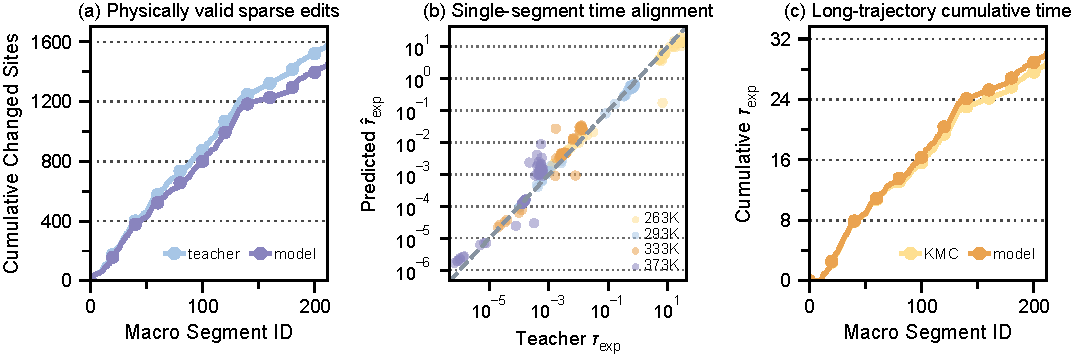
\includegraphics[width=0.92\linewidth]{fig/fig2_main_results.pdf}
  \caption{Controlled macro-step validation against the teacher simulator. The panels compare structural edit quality, projected validity, and expected-duration alignment under the same teacher-supervised segment protocol.}
  \label{fig:main-results}
\end{figure}

Given these paired macro segments, the first evaluation separates raw prediction quality from projection-closed physical validity. Sparse-edit metrics include change F1, top-$k$ change F1, projected change F1, changed-site type accuracy, projected changed-site type accuracy, reachability violation rate, mean vacancy transport cost, and projected global latent error; collection coverage, skipped no-op counts, and uncovered-segment counts keep candidate-support failures visible rather than absorbed into model accuracy. The expected-time head is evaluated against the path-conditioned CTMC target $\tau_{\mathrm{exp}}$ using log-MAE, log-RMSE, log-correlation, and scale ratio:
\begin{equation}
\mathrm{logMAE}_\tau
=
\frac{1}{N}\sum_{n=1}^{N}
\left|\log \hat{\tau}^{(n)}_{\mathrm{exp}}-\log \tau^{(n)}_{\mathrm{exp}}\right|,
\qquad
\mathrm{scale}_\tau
=
\frac{1}{N}\sum_{n=1}^{N}
\frac{\hat{\tau}^{(n)}_{\mathrm{exp}}}{\tau^{(n)}_{\mathrm{exp}}}.
\end{equation}
Scale ratio tests systematic time bias, and log-correlation tests relative variation across teacher segments. Because $\tau_{\mathrm{real}}$ is stochastic rather than the main macro-time target, the realized-time head is evaluated separately as an auxiliary lognormal distribution using NLL, 68\% and 95\% interval coverage, and probability-integral-transform diagnostics. Appendix~\ref{app:training-details} reports training parameters, compute resources, and runtime settings. Peak allocated GPU memory was not separately profiled; all runs fit within one 80 GB A100, with no multi-GPU or model-parallel execution.

\subsection{Closed-loop autonomous rollout, baselines, and ablations}

Paired evaluation verifies teacher-supervised segments but not compounding error when the student consumes its own predictions. We therefore use closed-loop rollout with an on-policy teacher-probe protocol: the model maintains autonomous state $\hat{X}_m$ by applying the previous projected sparse edit, while an evaluation-only KMC probe starts from the same $\hat{X}_m$, rolls forward for the selected horizon $k_m$, and provides a local state-time reference without overwriting the next student input. Thus the evaluated model trajectory is the closed-loop sequence
\(\hat{X}_0 \xrightarrow{k_0} \hat{X}_1 \xrightarrow{k_1} \cdots
\xrightarrow{k_{M-1}} \hat{X}_M\),
while each transition is scored against a KMC probe started from the current model state. This separates whether the student follows one stochastic KMC sample path from whether its self-generated macro trajectory remains locally reachable, inventory-preserving, temporally calibrated, and physically plausible under local probes; we use the latter as the closed-loop validity criterion.




Figure~\ref{fig:closed-loop-results} reports the Multi-K teacher-probe ablation matrices across Cu concentrations $0.005$ and $0.0134$ and temperatures $263$, $293$, $333$, and $373$K. Shared ablation rows and failure metrics isolate where edits may occur, how inventory is preserved, whether duration follows a path-conditioned CTMC target, and which learned components keep editable states stable.

\begin{figure}
  \centering
  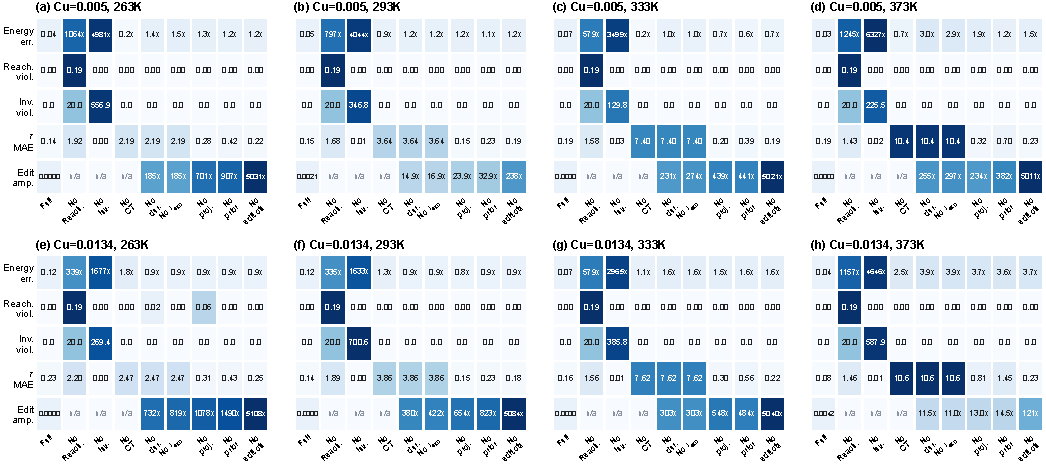
\includegraphics[width=0.92\linewidth]{fig/fig3_closed_loop_results.pdf}
  \caption{Cu-density and temperature ablation matrices for Multi-K teacher-probe rollout. Darker cells indicate larger failure.}
  \label{fig:closed-loop-results}
\end{figure}
These matrices use two non-learned references: the KMC teacher/reference supplies the rate-governed state-time target rather than a learned competitor, while the copy-state baseline keeps the lattice fixed and uses the CTMC start-state duration, preserving short-horizon scale from $R(X_t)$ but no structural evolution. The ablations are diagnostic: removing local reachability tests candidate-support necessity, removing inventory conservation tests material counts, and replacing learned duration with a start-state CTMC baseline tests path-conditioned information beyond local escape rate. Placing these failures beside the constrained model exposes each physical commitment instead of hiding violations in one accuracy number.
\subsection{Long-horizon diagnostics and efficiency}
After paired and closed-loop validity checks, Figure~\ref{fig:speedup-benchmark} reports timed end-to-end diagnostics over lattice size and temperature for replacing explicit micro-event replay with latent macro inference. Tens-to-hundreds-fold speedups come from expensive larger-scale KMC replay and AtomWorld-Mirror's reuse of learned local atomic physical regularities~\cite{plimpton1995fast,thompson2022lammps,li2019openkmc,zhang2018deeppotential,wang2018deepmdkit,batzner2022nequip,musaelian2023allegro}; the measurement includes benchmark orchestration around the macro world model, not only batched neural inference. Reported after validity and closed-loop checks, this timing tests replay reduction for a fixed workload only when edits remain reachable, inventory-preserving, and temporally calibrated, and it separates autonomous stability from teacher-forced duration/reward alignment.

Complementing autonomous rollout, a teacher-forced long-trajectory diagnostic queries state-conditioned time/reward alignment along a contiguous KMC trajectory. At segment $m$, from teacher state $X_{t_m}$, the model predicts a projected macro candidate; if several macro-step choices exist, the planner selects a legal one by the configured score; the teacher advances the matching microscopic dynamics to reference next state, reward, expected time, and realized time. The model contributes $(\Delta\hat{X}_m,\hat{\tau}_{\mathrm{exp},m},\hat{r}_m)$, while the evaluator reports cumulative expected-time curves, selected-horizon histograms, stop reasons, and cumulative energy-error summaries. This view does not claim the same stochastic micro-event path as KMC; it tests macro calibration on physically realized states, removing cumulative drift and isolating duration-scale errors, horizon-selection bias, and reward misalignment from distribution shift. The readout queries \(\{X_{t_m}\}_{m=0}^{M}\), where \(X_{t_m}\xrightarrow[\mathrm{teacher}]{k_m}X_{t_{m+1}}\), and accumulates predicted/reference expected times and the final clock-scale ratio:
\begin{equation}
\hat{T}^{\mathrm{exp}}_M=\sum_{m=0}^{M-1}\hat{\tau}_{\mathrm{exp},m},
\qquad
T^{\mathrm{exp}}_M=\sum_{m=0}^{M-1}\tau_{\mathrm{exp},m},
\qquad
\rho_T=\frac{\hat{T}^{\mathrm{exp}}_M}{T^{\mathrm{exp}}_M+\epsilon}.
\label{eq:teacher-forced-time-ratio}
\end{equation}

% This teacher-forced view has a narrower purpose than autonomous rollout. It does not claim that the model follows the same stochastic micro-event sample path as KMC; instead, it asks whether the macro predictor remains calibrated when queried along a physically realized trajectory. Because each query starts from an actual teacher state, cumulative drift is removed from the measurement, making duration scale errors, horizon-selection bias, and reward misalignment easier to isolate from state-distribution shift.
% The teacher-forced readout uses Equation~\eqref{eq:teacher-forced-path} for the queried teacher trajectory, Equation~\eqref{eq:teacher-forced-time} for accumulated predicted/reference expected time over the same selected horizons, and Equation~\eqref{eq:teacher-forced-ratio} for the final clock-scale ratio:
% \begin{align}
% X_{t_0} &\xrightarrow[\mathrm{teacher}]{k_0}X_{t_1}
% \xrightarrow[\mathrm{teacher}]{k_1}\cdots
% \xrightarrow[\mathrm{teacher}]{k_{M-1}}X_{t_M},\label{eq:teacher-forced-path}\\
% \hat{T}^{\mathrm{exp}}_M
% &=\sum_{m=0}^{M-1}\hat{\tau}_{\mathrm{exp},m},
% \qquad
% T^{\mathrm{exp}}_M=\sum_{m=0}^{M-1}\tau_{\mathrm{exp},m},\label{eq:teacher-forced-time}\\
% \rho_T&=\frac{\hat{T}^{\mathrm{exp}}_M}{T^{\mathrm{exp}}_M+\epsilon}.\label{eq:teacher-forced-ratio}
% \end{align}

\begin{figure}[H]
  \centering
  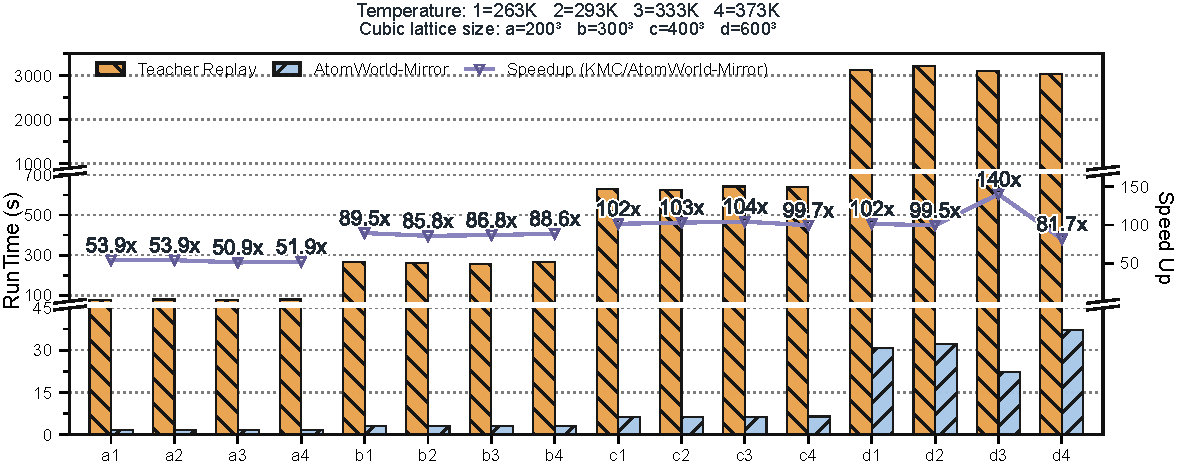
\includegraphics[width=0.92\linewidth]{fig/fig4_speedup_benchmark.pdf}
  \caption{End-to-end timing diagnostic across lattice sizes and temperatures.}
  \label{fig:speedup-benchmark}
\end{figure}

\FloatBarrier
\section{Related work}

Expanded comparisons are in Appendix~\ref{app:expanded-related-work}. Across atomistic dynamics simulation, existing acceleration often changes how trajectories are executed or coarse-grained rather than redefining what a learned model should predict: coarse-grained molecular dynamics and force matching map fine atoms or interactions into coarse beads or effective potentials, coarse-grained KMC and Monte Carlo aggregate microscopic cells, events, or occupancies, and Markov state models or state lumping cluster trajectory microstates into metastable macrostates and transition matrices~\cite{marrink2007martini,noid2008mscg,garnier2013cgkmc,chodera2014msm}. These methods abstract fine atoms, micro-events, or microstates into coarser units to reduce cost, but the retained states are usually determined by chosen coarse variables, metastability, or sampled transition statistics; they therefore do not explicitly identify whether evolution is moving in the right direction or which states form the critical evolution backbone. Learned potentials, graph/equivariant simulators, and physics-informed models show that reusable atomistic dynamics can be learned, while event-driven simulation, rare-event methods, and policy-guided search make trajectory traversal cheaper or more selective~\cite{behler2007nn,schutt2017schnet,batatia2022mace,zhang2018deeppotential,raissi2019pinn,pfaff2021meshgraphnets,bortz1975nfold,gillespie1977exact,li2019openkmc,voter1997hyperdynamics,schulman2017ppo,tang2024tks}; however, these lines generally target forces, dense states, local transition validation, or reward-shaped search rather than a reachable sparse macro edit with accumulated physical duration. AtomWorld-Mirror instead treats atomistic dynamics as a world-modeling problem: a simulator teacher, instantiated here by continuous-time KMC, supplies physical state-time supervision, while the Mirror learns consequential macro state-time transitions, so speedup comes from redesigning the predictive representation of atomic evolution rather than optimizing one simulator's event traversal.

\section{Conclusion}

We presented AtomWorld-Mirror, an atomistic world model that turns long-horizon simulation from exhaustive micro-event replay into predictive modeling of the critical evolution backbone. The central argument is that the bottleneck is representational as well as computational: conventional stepwise simulators treat transient fluctuations and persistent structural progress uniformly, while useful key states are defined by their predictive role in future evolution. AtomWorld-Mirror addresses this gap by mirroring AtomWorld in a backbone-aware latent space, where each macro rollout predicts a locally reachable sparse edit, preserves material inventory, and assigns the path-conditioned physical duration accumulated along the transition. The resulting speedup is therefore not a clock-only shortcut but a world-modeling speedup: low-impact intermediate resolution is removed while structurally valid state changes and continuous-time semantics are retained. Together, the implemented adaptive macro-step selection and long-horizon materials evolution results show that backbone-aware world modeling is already feasible under limited computational budgets, while broader simulator-teacher instantiations and alloy settings remain important extensions~\cite{jain2013materialsproject,merchant2023gnome,karniadakis2021piml}.

\newpage
{\small
\bibliographystyle{unsrtnat}
\bibliography{references}
}

\newpage
\appendix

\section{Training details and parameters}
\label{app:training-details}

\begin{table}[H]
  \caption{Training and evaluation configuration.}
  \label{tab:training-config}
  \centering
  \setlength{\tabcolsep}{3pt}
  \renewcommand{\arraystretch}{1.12}
  \begin{tabular}{@{}>{\raggedright\arraybackslash}p{0.17\linewidth} >{\raggedright\arraybackslash}p{0.28\linewidth} >{\raggedright\arraybackslash}p{0.18\linewidth} >{\raggedright\arraybackslash}p{0.27\linewidth}@{}}
    \toprule
    \textbf{Data / Teacher} & \textbf{Value} & \textbf{Student / Optim.} & \textbf{Value} \\
    \midrule
    \textbf{Teacher} & atom-vacancy KMC & \textbf{Student} & Dreamer world model \\
    \textbf{Lattice} & $40^3$ BCC & \textbf{Candidates} & 128 sites; 8 V seeds \\
    \textbf{Cu / V density} & 0.0134 / 0.0002 & \textbf{Path input} & teacher path summary \\
    \textbf{Temperature} & 300 K & \textbf{Latents} & global $32{\times}16$; patch/path 64/32 \\
    \textbf{Event support} & 2NN hops & \textbf{Epochs / batch} & 120 / 32 \\
    \textbf{Train / val} & 2000 / 400 segments per $k$ & \textbf{Optimizer} & Adam, lr $10^{-4}$ \\
    \textbf{Split policy} & independent envs & \textbf{Weight decay} & $10^{-5}$ \\
    \textbf{Filtering} & no-op skipped & \textbf{Time weights} & 1.0 / 0.25 \\
    \textbf{Time targets} & $\tau_{\mathrm{exp}}$ main; $\tau_{\mathrm{real}}$ aux & \textbf{Loss weights} & 0.5 / 0.5 / 0.25 / 0.25 \\
    \textbf{Aux. losses} & proj. / reward / priors & \textbf{Compute} & 1 A100; 35.5 min train; 23.3 / 47.1 s eval \\
    \bottomrule
  \end{tabular}
\end{table}

The reported training and evaluation runs use a single 80 GB A100 GPU, with no multi-GPU or model-parallel execution. The timing numbers above come from persisted run logs for the reported configuration; preliminary debugging and figure-style iterations are not part of the claimed experimental results.

\section{Cu--Fe alloy aging visualization}
\label{app:cu-cluster-evolution}

Figure~\ref{fig:cu-cluster-evolution} visualizes the initial and final Cu-cluster states in a Cu--Fe alloy aging simulation experiment. The KMC teacher trajectory uses the controlled binary-alloy setup from Section~4: a $40^3$ BCC lattice, Cu density $0.0134$, vacancy density $0.0002$, and vacancy-mediated 2NN event dynamics, and is rolled out for $50{,}000$ teacher micro-events. The full boxes show the whole simulated lattice state, while the partial boxes enlarge a representative sub-volume so that local Cu-cluster evolution is visible. Colors encode true Cu-cluster sizes computed on the full periodic BCC lattice by connecting Cu atoms through the teacher's 1NN/2NN neighborhood; the visualization therefore preserves the modest reorganization present in this teacher trajectory rather than artificially amplifying the before/after color contrast.

\begin{figure}[H]
  \centering
  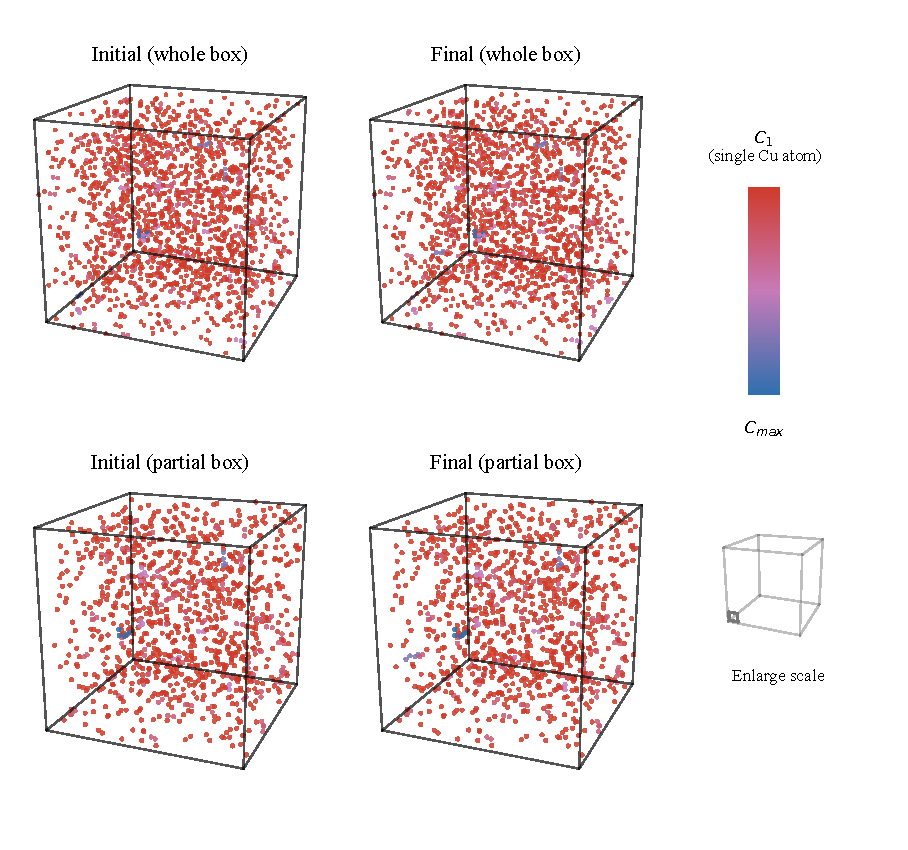
\includegraphics[width=0.92\linewidth]{fig/fig5_cu_cluster_evolution.pdf}
  \caption{Cu-cluster visual evolution from initial to final states in a Cu--Fe alloy aging simulation experiment. Each point denotes a Cu atom in the teacher-simulated lattice. Colors use a shared red--pink-purple--blue scale for the actual 1NN/2NN-connected Cu cluster size $C_i$, with red denoting single-Cu clusters and blue denoting the maximum cluster size in this trajectory.}
  \label{fig:cu-cluster-evolution}
\end{figure}

\section{Limitations and future work}
\label{app:limitations}

The present experiments focus on a binary Fe--Cu alloy system with vacancy-mediated atomic motion~\cite{soisson1996cufe,soisson2007cufe}. This controlled setting is useful for validating reachable sparse edits, inventory conservation, and continuous-time duration prediction, but real materials often involve more complex multi-component chemistries, including high-entropy alloys with richer local environments and competing diffusion pathways~\cite{yeh2004hea,cantor2004hea,miracle2017hea}. Future work should evaluate AtomWorld-Mirror on additional alloy families and extend the reachable edit-space construction and conservation projection to larger element inventories.

\section{Expanded related-work discussion}
\label{app:expanded-related-work}

Materials simulation already spans several representations of physical evolution rather than a single event-by-event execution model. Classical molecular dynamics advances atomic configurations by integrating many short time steps~\cite{alder1959md,rahman1964argon,verlet1967fluids,plimpton1995fast,thompson2022lammps}. Particle-based and continuum-scale simulation infrastructure further supports atomistic, mesoscopic, and field-level modeling within reusable materials codes~\cite{thompson2022lammps}. High-throughput materials databases and toolchains standardize structures, computed properties, and analysis workflows so that simulation outputs can be reused across discovery pipelines~\cite{jain2013materialsproject,curtarolo2012aflow,ong2013pymatgen,ward2018matminer,choudhary2020jarvis}. Because many simulators first choose a local update unit or a pre-defined state variable, a natural acceleration strategy is to lower resolution directly: coarse-grained molecular dynamics and force matching map multiple atoms into coarse beads or fit effective interactions~\cite{marrink2007martini,noid2008mscg}; coarse-grained KMC and Monte Carlo merge microscopic cells, events, or occupancies into coarser variables~\cite{garnier2013cgkmc}; and Markov state models or state lumping cluster trajectory microstates into metastable macrostates and transition matrices~\cite{chodera2014msm}. These abstractions reduce degrees of freedom, event counts, or state counts, and thereby make simulation cheaper. Their limitation for our purpose is not that they are invalid in their own regimes, but that reducing resolution is different from learning the predictive direction of evolution. They usually compress a trajectory after choosing a coarse representation or after observing sampled transitions; the importance of a state is then induced by the chosen coarse variables, metastability, or transition statistics rather than by its predicted role in future structural progress. AtomWorld-Mirror instead asks which future structural changes form the critical evolution backbone, whether the next macro state is worth advancing to, and how much physical time is accumulated along that transition.

Learning-based materials simulation has addressed this question by replacing or augmenting expensive local physics with learned representations. Neural-network potentials, Gaussian approximation potentials, graph neural networks, and equivariant force fields amortize energies, forces, and local structural regularities across atoms and molecules~\cite{behler2007nn,bartok2010gap,schutt2017schnet,xie2018cgcnn,batatia2022mace,gilmer2017mpnn,gasteiger2020dimenet,batzner2022nequip,musaelian2023allegro}. Deep potential molecular dynamics and related packages turn these learned local models into scalable dynamical simulators~\cite{zhang2018deeppotential,wang2018deepmdkit}. Physics-informed learning and graph-network simulators extend the same idea toward differential-equation, mesh-based, and interacting-system dynamics~\cite{raissi2019pinn,karniadakis2021piml,battaglia2016interaction,kipf2018nri,pfaff2021meshgraphnets}. These methods show that materials evolution can be learned at the level of reusable dynamics, not only as a faster implementation of an existing simulator. However, most of them target forces, fields, properties, or dense next-state evolution rather than a sparse macro state-time transition with an explicit physical clock.

Event-driven atomistic simulation provides the continuous-time teacher used in our experimental instantiation. Stochastic simulation and KMC sample local events from physical rates and advance a residence-time clock, which gives KMC its CTMC semantics~\cite{bortz1975nfold,gillespie1977exact,fichthorn1991dmc,chatterjee2007kmc}. These rate rules are local validators and clocks, not key-state selectors: they specify which microscopic updates are physically admissible and how time advances, but not whether the reached state should be retained as a useful waypoint for long-horizon evolution. High-performance KMC systems such as OpenKMC use carefully engineered parallel execution to reach very large systems~\cite{li2019openkmc}, while rare-event and accelerated-dynamics methods reduce slow-transition costs through known barriers, metastable states, bias potentials, path ensembles, or state partitions~\cite{voter1997hyperdynamics,voter1998parallelreplica,sorensen2000tad,henkelman2000neb,henkelman2001akmc,laio2002metadynamics,bolhuis2002tps,zamora2016spectad,liu2023trps,lin2019partialscaling}. PPO-style policy optimization, reinforcement-learning-guided long-timescale transport simulation, and policy-guided Monte Carlo can further bias action selection toward reward, transport, or path discovery~\cite{schulman2017ppo,tang2024tks,bojesen2018pgmc}. When the reward emphasizes rapid energy decrease or another user-chosen objective, such policies can preferentially search for the steepest predicted improvement path. This may be useful as an optimization heuristic, but the resulting trajectory is policy-shaped rather than rate-shaped: it can distort the natural evolution of the atomic world and cannot by itself inherit a simulator's physical clock, which reduces its usefulness for time-resolved materials prediction. These approaches make event-level exploration cheaper or more selective, but they do not by themselves define a learned macro world model whose rollout unit is a reachable sparse edit together with accumulated physical duration. AtomWorld-Mirror is positioned at this representation level: a rate-governed simulator teacher, instantiated here by KMC, provides the controlled state-time reference, while the student learns teacher-supervised macro state-time transitions along the critical evolution backbone. Speedup therefore comes from changing the predictive representation of atomistic dynamics, not from optimizing one simulator's event traversal or discarding physical time.

\newpage
\input{checklist.tex}

\end{document}
